\chapter{Analiza nawiązanej komunikacji}
    \begin{figure}[h!]
        \centering
        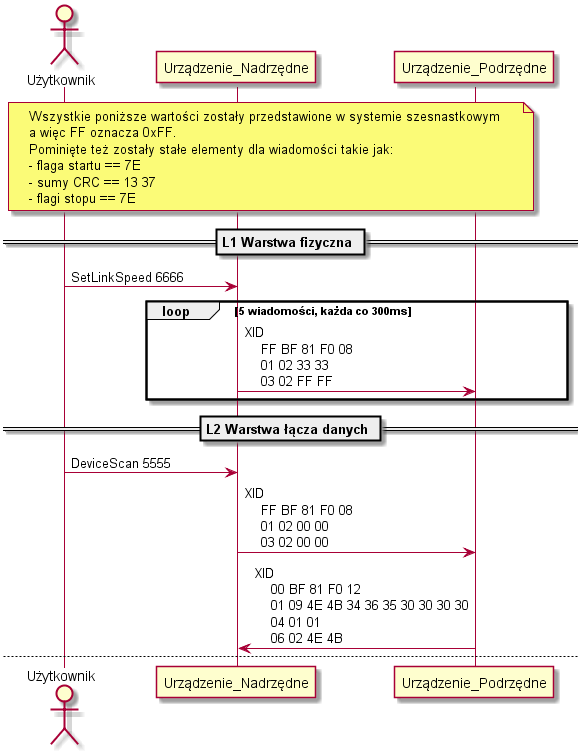
\includegraphics[scale=0.70]{out/Diagramy/UML_DiagramOfSequence_New/UML_DiagramOfSequence_New-page1.png}
        \caption{Ustanowienie prędkości połączenia wraz z początkowym skanowaniem urządzeń
            \newline(Opracowanie własne)}
        \label{fig:DiagramSequence_LinkSpeed_DeviceScan}
        \end{figure}
    \newpage
    W celu szczegółowej analizy wykonania programu przedstawionego na listingu \ref{lst:WykonanieProgramu}, utworzono diagram sekwencji podzielony na kilka części 
    (rysunek \ref{fig:DiagramSequence_LinkSpeed_DeviceScan}),
    co pozwoliło zobrazować zaistniałą komunikację pomiędzy użytkownikiem, urządzeniem nadrzędnym oraz urządzeniem podrzędnym.
    Na diagramie oraz podczas analizy pominięto cztery bajty stałe dla każdej wiadomości, czyli bajt startu równy 0x7E, dwa bajty sumy CRC =\{ 0x13, 0x37\} ( powód dlaczego ta wartość jest stała przedstawiono
    w podsumowaniu ) oraz bajt stopu równy 0x7E.

%%%%%%%%%%%%%%%%%%%%%%%%%%%%%%%%%%%%%%%%%%%%%%%%%%%%%%%%%%%%%%%%%%%%%%%%%%%%%%%%%%%%%%%%%%%%%%%%%%%%%%%%%%%%%%%%%%%%%%%%%

\section{Ustanowienie prędkości połączenia}
Parametrem tej komendy jest adres portu 6666, z którego korzysta sterownik do nawiązania połączenia typu tcp na adresie 127.0.0.1 wraz z symulatorem urządzenia
przy zastosowaniu wzorca Publikuj-Subskrybuj. Podczas tego połączenia protokół AISG 2.0 nie zakłada oczekiwania na odpowiedź od urządzenia podrzędnego oraz użyta biblioteka
ZeroMQ również nie udostępnia możliwości wysłania odpowiedzi na taką wiadomość.
\newline\newline
Analiza wartości wiadomości wychodzącej (rysunek \ref{lst:WykonanieProgramu}- linijki [3; 12]):
\begin{enumerate}
    \item ADDR = 0xFF --- \textit{broadcast};
    \item CTRL = 0xBF --- charakterystyczny dla ramki XID;
    \item FI = 0x81 --- charakterystyczna dla ramki XID oraz grupy wiadomości przypisania adresu;
    \item GI = 0xF0 --- grupa wiadomości przypisania adresu;
    \item GL = 0x08;
\end{enumerate}
Analizę kolejnych bajtów tej wiadomości pominięto, ponieważ mogą one przyjmować dowolną wartość. 

%%%%%%%%%%%%%%%%%%%%%%%%%%%%%%%%%%%%%%%%%%%%%%%%%%%%%%%%%%%%%%%%%%%%%%%%%%%%%%%%%%%%%%%%%%%%%%%%%%%%%%%%%%%%%%%%%%%%%%%%%

\section{Skanowanie urządzeń}
Parametrem tej komendy jest adres portu 5555, z którego korzysta sterownik
do nawiązania połączenia typu tcp na adresie 127.0.0.1 wraz z symulatorem urządzenia,
przy zastosowaniu wzorca Żadanie-Odpowiedź. Jest to wzorzec, który zakłada otrzymanie odpowiedzi na każdą wysłaną wiadomość, zanim kolejna zostanie nadana. 
Opisany mechanizm komunikacji aplikowalny jest również do wszystkich poniższych komend.
\newline\newline
Analiza wartości wiadomości wychodzącej 
(rysunek \ref{lst:WykonanieProgramu} - linijki {15, 16}, rysunek \ref{fig:DiagramSequence_LinkSpeed_DeviceScan}):
\begin{enumerate}
    \item ADDR = 0xFF --- broadcast;
    \item CTRL = 0xBF --- charakterystyczny dla ramki XID;
    \item FI = 0x81 --- charakterystyczna dla ramki XID oraz grupy wiadomości przypisania adresu;
    \item GI = 0xF0 --- grupa wiadomości przypisania adresu;
    \item GL = 0x08;
    \item Pierwszy parametr HDLC:
    \begin{enumerate}
        \item PI = 0x01 --- unikalny identyfikator urządzenia podrzędnego;
        \item PL = 0x02;
        \item PV = \{ 0x00, 0x00 \} --- zestawienie tych wartości spowoduje, że każde urządzenie podłączone do portu zgłosi swoją obecność;
    \end{enumerate}
    \item Drugi parametr HDLC:
    \begin{enumerate}
        \item PI = 0x03 --- maska unikalnego identyfikatora;
        \item PL = 0x02;
        \item PV = \{ 0x00, 0x00 \}  --- zestawienie tych wartości spowoduje, że każde urządzenie podłączone do portu zgłosi swoją obecność;
    \end{enumerate}
\end{enumerate}
\bigskip
Analiza wartości wiadomości przychodzącej 
(rysunek \ref{lst:WykonanieProgramu}- linijka 17, rysunek \ref{fig:DiagramSequence_LinkSpeed_DeviceScan}):
\begin{enumerate}
    \item ADDR = 0x00 --- urządzenie podrzędne jest jest w stanie niezaadresowanym;
    \item CTRL = 0xBF --- charakterystyczny dla ramki XID;
    \item FI = 0x81 --- charakterystyczna dla ramki XID oraz grupy wiadomości przypisania adresu;
    \item GI = 0xF0 --- grupa wiadomości przypisania adresu;
    \item GL = 0x12;
    \item Pierwszy parametr HDLC:
    \begin{enumerate}
        \item PI = 0x01 --- unikalny identyfikator urządzenia podrzędnego;
        \item PL = 0x09;
        \item PV = \{ 0x4E, 0x4B, 0x34, 0x36, 0x35, 0x30, 0x30, 0x30, 0x30 \};
    \end{enumerate}
    \item Drugi parametr HDLC:
    \begin{enumerate}
        \item PI = 0x04 --- typ urządzenia podrzędnego;
        \item PL = 0x01;
        \item PV = 0x01 --- pojedynczy RET;
    \end{enumerate}
    \item Trzeci parametr HDLC:
    \begin{enumerate}
        \item PI = 0x06 --- kod producenta urządzenia podrzędnego;
        \item PL = 0x02;
        \item PV = \{ 0x4E, 0x4B \};
    \end{enumerate}
\end{enumerate}

%%%%%%%%%%%%%%%%%%%%%%%%%%%%%%%%%%%%%%%%%%%%%%%%%%%%%%%%%%%%%%%%%%%%%%%%%%%%%%%%%%%%%%%%%%%%%%%%%%%%%%%%%%%%%%%%%%%%%%%%%

\section{Żadanie adresacji}
Tutaj po raz pierwszy można zaobserwować zmienioną wartość pola adresu dla wiadomości
przychodzącej. Oznacza to, że urządzenie podrzędne zaakceptowało żadanie adresacji 
oraz identyfikuje się w trakcie rozmowy z urządzeniem nadrzędnym pod adresem 0x03 co
jest prawdą dla każdej następnej wiadomości.
\newline\newline
Analiza wartości wiadomości wychodzącej 
(rysunek \ref{lst:WykonanieProgramu}, linijki {20, 21} oraz \ref{fig:DiagramSequence_AddressAssignment_SecondDeviceScan}):
\begin{enumerate}
    \item ADDR = 0xFF --- broadcast;
    \item CTRL = 0xBF --- charakterystyczny dla ramki XID;
    \item FI = 0x81 --- charakterystyczna dla ramki XID oraz grupy wiadomości przypisania adresu;
    \item GI = 0xF0;
    \item GL = 0x11;
    \item Pierwszy parametr HDLC:
    \begin{enumerate}
        \item PI = 0x01 --- unikalny identyfikator urządzenia podrzędnego;
        \item PL = 0x09;
        \item PV = \{ 0x4E, 0x4B, 0x34, 0x36, 0x35, 0x30, 0x30, 0x30, 0x30 \};
    \end{enumerate}
    \item Drugi parametr HDLC:
    \begin{enumerate}
        \item PI = 0x02 --- docelowy adres urządzenia podrzędnego;
        \item PL = 0x01;
        \item PV = 0x03;
    \end{enumerate}
    \item Trzeci parametr HDLC:
    \begin{enumerate}
        \item PI = 0x04 --- typ urządzenia podrzędnego;
        \item PL = 0x01;
        \item PV = 0x01 --- pojedynczy RET;
    \end{enumerate}
\end{enumerate}
\bigskip
Analiza wartości wiadomości przychodzącej 
(rysunek \ref{lst:WykonanieProgramu}- linijka 22, rysunek \ref{fig:DiagramSequence_AddressAssignment_SecondDeviceScan}):
\begin{enumerate}
    \item ADDR = 0x03 --- urządzenie identyfikuje się żądanym adresem;
    \item CTRL = 0xBF --- charakterystyczny dla ramki XID;
    \item FI = 0x81 --- charakterystyczna dla ramki XID oraz grupy wiadomości przypisania adresu;
    \item GI = 0xF0;
    \item GL = 0x12;
    \item Pierwszy parametr HDLC:
    \begin{enumerate}
        \item PI = 0x01 --- unikalny identyfikator urządzenia podrzędnego;
        \item PL = 0x09;
        \item PV = \{ 0x4E, 0x4B, 0x34, 0x36, 0x35, 0x30, 0x30, 0x30, 0x30 \};
    \end{enumerate}
    \item Drugi parametr HDLC:
    \begin{enumerate}
        \item PI = 0x04 --- typ urządzenia podrzędnego;
        \item PL = 0x01;
        \item PV = 0x01 --- pojedynczy RET;
    \end{enumerate}
    \item Trzeci parametr HDLC:
    \begin{enumerate}
        \item PI = 0x06 --- kod producenta urządzenia podrzędnego;
        \item PL = 0x02;
        \item PV = \{ 0x4E, 0x4B \};
    \end{enumerate}
\end{enumerate}

\begin{figure}[h!]
    \centering
    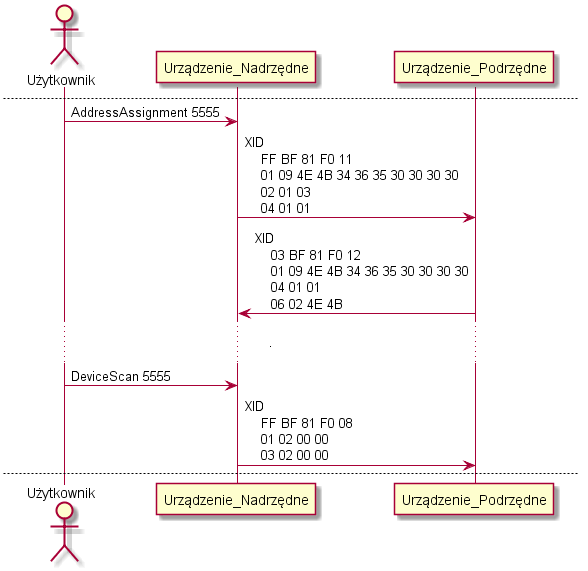
\includegraphics[scale=0.75]{out/Diagramy/UML_DiagramOfSequence_New/UML_DiagramOfSequence_New-page2.png}
    \caption{Żadanie adresacji oraz dodatkowe skanowanie urządzeń.
        \newline(Opracowanie własne)}
    \label{fig:DiagramSequence_AddressAssignment_SecondDeviceScan}
\end{figure}

%%%%%%%%%%%%%%%%%%%%%%%%%%%%%%%%%%%%%%%%%%%%%%%%%%%%%%%%%%%%%%%%%%%%%%%%%%%%%%%%%%%%%%%%%%%%%%%%%%%%%%%%%%%%%%%%%%%%%%%%%

\section{Ponowne skanowanie urządzeń}
Na rysunku \ref{fig:DiagramSequence_AddressAssignment_SecondDeviceScan} przedstawiono ponowne żądanie skanowania urządzenia na linii.
Zostało to wykonane w celu upewnienia się, że poprzednia procedura adresacji powiodła się. Po zaadresowaniu urządzenia podrzędnego, nie powinno
ono odpowiedzieć na wiadomość typu broadcast.

%%%%%%%%%%%%%%%%%%%%%%%%%%%%%%%%%%%%%%%%%%%%%%%%%%%%%%%%%%%%%%%%%%%%%%%%%%%%%%%%%%%%%%%%%%%%%%%%%%%%%%%%%%%%%%%%%%%%%%%%%

\section{Negocjacje parametrów HDLC}
Cechą negocjacji parametrów przy pomocy ramek XID jest to, że jeśli żądana wartość jest wspierana przez
urządzenie podrzędne, to odpowie ono wiadomością zawierającą te same parametry oraz te same wartości. 
W przeciwnym wypadku otrzymanymi wartościami parametrów będą największe możliwe przez nie wspierane.
Zaobserwowano to zjawisko w przypadku negocjacji wielkości payloadu dla wysłanej oraz otrzymanej ramki informacyjnej.
\newline\newline
Analiza wartości wiadomości wychodzącej 
(rysunek \ref{lst:WykonanieProgramu}, linijki {30, 31} oraz \ref{fig:DiagramSequence_HDLCParameters_SNRM}):
\begin{enumerate}
    \item ADDR = 0x03 --- adres nadany urządzeniu podrzędnemu;
    \item CTRL = 0xBF --- charakterystyczny dla ramki XID;
    \item FI = 0x81 --- charakterystyczna dla ramki XID oraz grupy wiadomości przypisania adresu;
    \item GI = 0xF0;
    \item GL = 0x12;
    \item Pierwszy parametr HDLC:
    \begin{enumerate}
        \item PI = 0x05 --- maksymalny rozmiar payloadu wysyłanej ramki I;
        \item PL = 0x04;
        \item PV = \{0xF0, 0x2D, 0x00, 0x00\} czyli 61485 bity;
    \end{enumerate}
    \item Drugi parametr HDLC:
    \begin{enumerate}
        \item PI = 0x06 --- maksymalny rozmiar payloadu odbieranej ramki I;
        \item PL = 0x04;
        \item PV = \{0xF0, 0x2D, 0x00, 0x00\} czyli 61485 bity;
    \end{enumerate}
    \item Trzeci parametr HDLC:
    \begin{enumerate}
        \item PI = 0x07 --- maksymalna liczba ramek wysłanych pod rząd;
        \item PL = 0x01;
        \item PV = 0x01;
    \end{enumerate}
    \item Czwarty parametr HDLC:
    \begin{enumerate}
        \item PI = 0x08 --- maksymalna liczba ramek odebranych pod rząd;
        \item PL = 0x01;
        \item PV = 0x01;
    \end{enumerate}
\end{enumerate}
\bigskip
Analiza wartości wiadomości przychodzącej 
(rysunek \ref{lst:WykonanieProgramu}- linijka 32, rysunek \ref{fig:DiagramSequence_HDLCParameters_SNRM}):
\begin{enumerate}
    \item ADDR = 0x03 --- urządzenie identyfikuje się żądanym adresem;
    \item CTRL = 0xBF --- charakterystyczny dla ramki XID;
    \item FI = 0x81 --- charakterystyczna dla ramki XID oraz grupy wiadomości przypisania adresu;
    \item GI = 0x80;
    \item GL = 0x12;
    \item Pierwszy parametr HDLC:
    \begin{enumerate}
        \item PI = 0x05 --- maksymalny rozmiar payloadu wysyłanej ramki I;
        \item PL = 0x04;
        \item PV = \{0x50, 0x02, 0x00, 0x00\} czyli 20482 bity
    \end{enumerate}
    \item Drugi parametr HDLC:
    \begin{enumerate}
        \item PI = 0x06 --- maksymalny rozmiar payloadu odbieranej ramki I;
        \item PL = 0x04;
        \item PV = \{0x50, 0x02, 0x00, 0x00\} czyli 20482 bity
    \end{enumerate}
    \item Trzeci parametr HDLC:
    \begin{enumerate}
        \item PI = 0x07 --- maksymalna liczba ramek wysłanych;
        \item PL = 0x01;
        \item PV = 0x01;
    \end{enumerate}
    \item Czwarty parametr HDLC:
    \begin{enumerate}
        \item PI = 0x08 --- maksymalna liczba ramek odebranych;
        \item PL = 0x01;
        \item PV = 0x01;
    \end{enumerate}
\end{enumerate}

%%%%%%%%%%%%%%%%%%%%%%%%%%%%%%%%%%%%%%%%%%%%%%%%%%%%%%%%%%%%%%%%%%%%%%%%%%%%%%%%%%%%%%%%%%%%%%%%%%%%%%%%%%%%%%%%%%%%%%%%%

\section{Przejście na normalny tryb odpowiedzi}
Normalny tryb odpowiedzi to jest taki, w którym urządzenie podrzędne nie może inicjować transmisji.
Analiza wartości wiadomości wychodzącej 
(rysunek \ref{lst:WykonanieProgramu}, linijki 35, 36 oraz \ref{fig:DiagramSequence_HDLCParameters_SNRM}):
\begin{enumerate}
    \item ADDR = 0x03 --- adres nadany urządzeniu podrzędnemu;
    \item CTRL = 0x93 --- charakterystyczny dla ramki U, SNRM;
\end{enumerate}
\bigskip
Analiza wartości wiadomości przychodzącej
(rysunek \ref{lst:WykonanieProgramu}, linijka 37 oraz \ref{fig:DiagramSequence_HDLCParameters_SNRM}):
\begin{enumerate}
    \item ADDR = 0x03 --- adres nadany urządzeniu podrzędnemu;
    \item CTRL = 0x73 --- charakterystyczny dla ramki U, UA;
\end{enumerate}

%%%%%%%%%%%%%%%%%%%%%%%%%%%%%%%%%%%%%%%%%%%%%%%%%%%%%%%%%%%%%%%%%%%%%%%%%%%%%%%%%%%%%%%%%%%%%%%%%%%%%%%%%%%%%%%%%%%%%%%%%

\section{Wersja standardu 3GPP}
Ciekawą obserwacją tej wiadomości jest fakt, że identyfikator parametru równy 0x05 pojawił się podczas definiowania długości payloadu
dla ramki informacyjnej. Różnica polega na tym, że tamta wiadomość posiadała identyfikator grupy równy 0x80
\newline\newline
Analiza wartości wiadomości wychodzącej 
(rysunek \ref{lst:WykonanieProgramu}, linijki {40, 41} oraz \ref{fig:DiagramSequence_3GPP_AISGVersion_Calibrate}):
\begin{enumerate}
    \item ADDR = 0x03 --- adres nadany urządzeniu podrzędnemu;
    \item CTRL = 0xBF --- charakterystyczny dla ramki XID;
    \item FI = 0x81 --- charakterystyczna dla ramki XID oraz grupy wiadomości przypisania adresu;
    \item GI = 0xF0;
    \item GL = 0x03;
    \item Parametr HDLC:
    \begin{enumerate}
        \item PI = 0x05 --- wersja standardu 3GPP;
        \item PL = 0x01;
        \item PV = 0x08 --- pionierska dla technologii LTE
    \end{enumerate}
\end{enumerate}
Wiadomość przychodząca posiada tę samą wartość co wychodząca, dlatego pominięto jej analizę.

%%%%%%%%%%%%%%%%%%%%%%%%%%%%%%%%%%%%%%%%%%%%%%%%%%%%%%%%%%%%%%%%%%%%%%%%%%%%%%%%%%%%%%%%%%%%%%%%%%%%%%%%%%%%%%%%%%%%%%%%%

\section{Wersja protokołu AISG}
Analiza wartości wiadomości wychodzącej 
(rysunek \ref{lst:WykonanieProgramu}, linijki {45, 46} oraz \ref{fig:DiagramSequence_3GPP_AISGVersion_Calibrate}):
\begin{enumerate}
    \item ADDR = 0x03 --- adres nadany urządzeniu podrzędnemu;
    \item CTRL = 0xBF --- charakterystyczny dla ramki XID;
    \item FI = 0x81 --- charakterystyczna dla ramki XID oraz grupy wiadomości przypisania adresu;
    \item GI = 0xF0;
    \item GL = 0x03;
    \item Parametr HDLC:
    \begin{enumerate}
        \item PI = 0x14 --- wersja protokołu AISG;
        \item PL = 0x01;
        \item PV = 0x02 --- wybrano wersję v2.0, istnieją jeszcze: 1.0, 1.1 oraz 3.0
    \end{enumerate}
\end{enumerate}
Wiadomość przychodząca posiada tę samą wartość co wychodząca, dlatego pominięto jej analizę.
